\chapter{Introduction\label{chap:intro}}

% Being upfront: What is this thesis about?
In this thesis, we propose an algorithmic approach for exactly solving \NP-hard optimization problems with two conflicting objectives.
The algorithm proposed is based on declarative programming and is generally applicable to problems that can easily represented in propositional logic because it works in the declarative paradigm of propositional satisfiability.

% What are optimization problems and where do they occur
% Start by telling a story (running example throughout intro)
When one is looking for a new flat to buy, most people will be comparing prices with the aim to find the cheapest flat possible that fulfils their requirements.
This is an example of what are called optimization problems.
Optimization problems can be summarized as the task of finding a ``best'' solution out of a collection of possible solutions available.
Commonly, the notion of ``best'' that is used in optimization is that a solution of minimum associated ``cost'' is considered optimal.
Speaking in the example from above, the task is to find the flat from all flats that fulfils the requirements for the cheapest price.
If the collection of possible solutions is discrete (as in the flat example), we speak of \emph{combinatorial} optimization.

% Applications of optimization in literature
Combinatorial optimization problems naturally arise in many areas, ranging from industrial applications over research to everyday tasks.
Examples in literature include scheduling~\autocites{DBLP:conf/cp/Stojadinovic14,DBLP:conf/cpaior/BofillGSV15,DBLP:journals/ior/Solomon87,DBLP:journals/candie/AkyolB07}, supply chain optimization~\autocite{}, minimizing the loss of a neural network~\autocite{}, air traffic management~\autocites{DBLP:journals/ior/BertsimasLO11,RichardsHow2002Aircrafttrajectoryplanning}, clustering~\autocite{DBLP:journals/ai/DaoDV17,DBLP:conf/sdm/DavidsonRS10}, learning optimal classifiers~\autocites{DBLP:conf/cp/MaliotovM18,DBLP:conf/ijcai/NarodytskaIPM18,DBLP:conf/ijcai/Hu0HH20,DBLP:conf/cp/YuISB20,DBLP:conf/aaai/DemirovicS21,DBLP:conf/cp/ShatiCM21} and many more.

% Hardness of optimization problems
In the same way that there are different complexity classes for decision problems, these complexity classes can be extended to optimization problems as well.
Probably the two most important complexity classes are $\mathcal{P}$ and \NP.
$\mathcal{P}$ contains all problems for which an algorithm that solves the problem in polynomial time is known.
For problems in \NP, on the other hand, to our current knowledge, no such algorithm exists.
This means that the worst case runtime for \NP-complete (i.e., exactly as hard as the hardest problems in \NP) and \NP-hard (i.e., at least as hard as problems in \NP) problems is exponential.
Consider the \NP-complete~\autocite{} set covering decision problem~\autocite{DBLP:conf/coco/Karp72} where for a collection $\sets$ of sets, the task is to determine whether a cover $\cover$ with cardinality smaller than a threshold $k$ exists so that the cover intersects all sets, i.e., $S \cap \cover \neq \emptyset$ for all $S\in\sets$.
The corresponding optimization problem, where the task is to find the \emph{smallest} such cover is \NP-hard.
Several well known \NP-complete decision problems have corresponding \NP-hard optimization problems~\autocite{KorteVygen2018-15}.

% Approaches to solving optimization
Since there is such a variety of applications for combinatorial optimization, a plethora of algorithmic approaches to solving optimization problems have been proposed.
These approaches range from stochastic local search~\autocite{}, over evolutionary~\autocites{Dasgupta2013,DBLP:journals/jgo/StornP97} to algorithms based on declarative programming~\autocite{}.
In addition to these generally applicable approaches, there are problem specific algorithms, e.g., based on dynamic programming~\autocite{DBLP:conf/aaai/DemirovicS21}\TODO{more examples}.
One other attribute on which the optimization approaches differ is whether they are exact or approximative, meaning if they are guaranteed to find \emph{the best} or \emph{a good} solution to any instance (given enough resources).
Even though some others are also briefly surveyed in a later chapter, this work mainly focuses on declarative (and therefore general) and exact approaches.

% Solving pipeline for declarative approaches
In the declarative approach to solving optimization problems, the problem of interest is first \emph{encoded} into a declarative programming language of choice.
Examples of declarative languages are maximum satisfiability~\autocite{handbook2-maxsat}, constraint programming~\autocite{} and mixed integer linear programming~\autocites{ChenEtAl2010-intro,KorteVygen2018-5}.
An encoding is hereby a mapping of the original problem to a problem in the declarative language, where each optimal solution to the encoded instance corresponds to an optimal solution of the original problem.
The choice of declarative language should be based on what the problem of interested can be naturally encoded in.
Next, a general optimization solver for the chosen declarative language is used to solve the encoded problem to obtain on optimal solution for it.
A solver for a declarative programming language is an algorithm that finds an optimal solution to an optimization instance in a declarative programming language.
The last step is to map this solution back to the original problem space.
This solving pipeline of the declarative approach to optimization is illustrated in \cref{fig:solving-pipeline}.

\begin{figure}
  \centering
  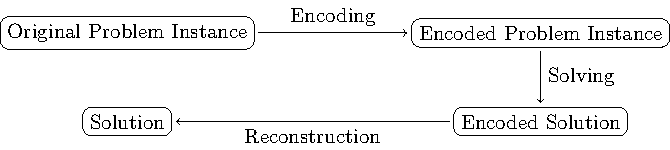
\includegraphics{solving-pipeline.pdf}
  \caption{The solving pipeline of the declarative approach to optimization.}\label{fig:solving-pipeline}
\end{figure}

% Advantages of declarative approaches
The advantage of declarative approaches is that the solving algorithm itself is general and can be used for different problems, as long as \TODO{a polynomial size encoding (rephrase as ``an encoding of size that doesn't influence runtime'')} exists.
The task of applying a given declarative method to a new problem consists therefore in finding an encoding and not in coming up with a new algorithm.
Furthermore, improvement that is made in developing solvers for the declarative language immediately maps to better solving performance for \emph{all} problems that can be encoded into this declarative language.

% Runtimes in declarative approaches
In the scope of this work, we focus on using declarative approaches for solving \NP-hard optimization problems.
For this application, \NP-hard declarative languages are used, meaning the generic solving step is the only computationally hard step in the solving pipeline.
Both the encoding and the reconstruction of the solution are typically done in polynomial time.
Since the declarative language is \NP-hard (assuming $\mathcal{P}\neq\mathcal{NP}$), the worst-case runtime of the solving algorithm cannot be better than exponential.
However, in practice one can observe significantly better performance from many solving algorithms for ``interesting'' instances, i.e., instances that appear for real-world problems.
Examples for solving algorithms for \NP-hard declarative languages that achieve good performance on real-world instances are conflict driven clause learning solvers for propositional satisfiability~\autocite{handbook2-cdcl} and state-of-the-art branch-and-cut algorithms for mixed integer linear programming~\autocite{ChenEtAl2010-branch-and-cut}.

% Reveal conflicting second objective
Taking a closer look at the flat search example from the beginning, we can notice a problem emerging:
what does ``fulfilling'' the requirements mean?
Some requirements, like the number of rooms, might be easy to specify, but consider the distance of ones daily commute.
Rather than setting a fixed threshold as ``maximum $x$ kilometres distance'', what we might actually want to do is minimize this distance at the same time as the cost of the flat.
Now there are multiple objectives to take into account regarding what constitutes a ``best'' solution.
Multiple objectives give rise to \emph{multi-objective} optimization.

% Conflicting objectives and why there might be no single optimal solution
A crucial difference between single-objective and multi-objective optimization is that there is no single notion of optimality for the multi-objective setting.
Whereas for a single objective function, there is a clear minimum (or maximum) and objective values can be unambiguously compared, this becomes less defined for the multi-objective case:
consider a flat with a cost of 300\,000 \texteuro{} and 4-kilometre daily commute and compare it to another flat that costs 240\,000 \texteuro{} and has a 3-kilometre daily commute.
In this case it is easy to say that the second option is more optimal.
However, compare the second option to another flat that costs 270\,000 \texteuro{} but only has a 1-kilometre daily commute.
Now, it is not any more immediately clear which one of these options is better, and the choice would depend on ones personal preference over the two objectives.
This becomes especially difficult if there is no clear preference over the objectives.
Typically, a situation like that occurs when two of the objectives considered are in conflict, as the price of a flat and the corresponding daily commute might be if the commute is towards the city centre and flats in the city centre are more expensive.

% Pareto optimality
% Point out different nomenclature
In the context of our work, the notion of optimality for multi-objective optimization is that of Pareto optimality (also called efficiency in other contexts)~\autocite{Ehrgott2005-2}.
Intuitively, Pareto optimality considers a solution optimal if there are no other solutions with better objective values for one objective and not worse for all the others. 
This definition would consider the two last flats from earlier both equally optimal.
Under Pareto optimality, the task of solving a multi-objective optimization problem can mean multiple things:
finding a single Pareto-optimal solution, finding a representative solution for each Pareto point (also called non-dominated point in literature~\autocite{Ehrgott2005-2}), or finding all Pareto-optimal solutions.
The first of the tasks can be considered the least informative since there can be very different Pareto-optimal solutions to the same problem.
Most approaches to solving multi-objective optimization under Pareto optimality seem to focus on the second approach where a single solution per Pareto point (i.e., tuple of Pareto-optimal objective values) is computed.
This gives a human decision maker the ability to look at the results and choose the Pareto-optimal solution that gives the best trade-off between the objectives after the fact instead of having to choose such a trade-off in advance.
The last task goes one step further and enumerates the full Pareto front (i.e., all Pareto-optimal solutions), even if multiple of the solutions might lead to the same objective values.
In this work we focus on the latter two tasks.

% Bi-objective vs multi-objective
% Why bi-objective is interesting/enough
The handle on multiple objectives and what the objective values of an optimal solution actually mean can quickly become hard to grasp.
As humans, we can only visualize three dimensions meaning a Pareto front over four objectives is already an entirely abstract object while even a three-dimensional one is hard to visualize.
Imagine, for example, adding the objectives living space and renovations that need to be done into the flat search example.
With those four objectives, a lot more flats are going to be Pareto-optimal and the set of Pareto-optimal solutions becomes less helpful for making a decision.
Two objectives, however, form a good trade-off between gaining meaningful information from the second objective over just using a single one, being able to intuitively visualize the Pareto front and not resulting in too many Pareto-optimal solutions.
Additionally, objectives that are considered ``less important'' but should still somehow be included in the optimization can still be added as a threshold condition;
e.g., requiring that the living space is more than 60 $\text{m}^2$ rather than treating it as a separate objective.
In this work we focus on \emph{bi-objective} optimization and develop an algorithm for finding either a single representative per Pareto point or all Pareto-optimal solutions.

% Applications of bi-objective optimization in literature
Bi-objective optimization problems also arise naturally in many fields of application.
In machine learning, a regularization term---expressing how complex a certain model is---is often combined with the loss based on the classification error~\autocite{}.
Typically, this is done by forming a linear combination of the two components, but there is also research in treating the two objectives separately~\autocite{DBLP:journals/tsmc/JinS08}.
A very similar idea can be used for learning interpretable machine learning models.
As a proxy for the objective of interpretability, typically a notion of ``size'' of the model is used, leading to a natural bi-objective optimization problem with the objectives classification error and model size~\autocites{DBLP:conf/ijcai/Ignatiev0NS21,DBLP:conf/cp/MaliotovM18,DBLP:conf/ijcai/NarodytskaIPM18,DBLP:conf/ijcai/Hu0HH20,DBLP:conf/cp/YuISB20,DBLP:conf/aaai/Ignatiev0S021}.
A bi-objective optimization problem also arises when wanting to create a portfolio of different solvers that together solve a set of benchmarks as fast as possible while also containing as few solvers as possible~\autocite{DBLP:conf/cp/JanotaMSM21}.
There are also bi-objective optimization problems in network routing with the objectives load balancing and latency~\autocite{SilverioEtAl2022biobjectiveoptimization}.
In supply chain optimization, in addition to the economic objective, environmental aspects can be taken into consideration as a second objective~\autocite{DBLP:journals/cce/Pinto-VarelaBN11}.

% MaxSAT (and SAT)
In this work, we focus on maximum satisfiability (MaxSAT) as the declarative approach for solving optimization problems.
MaxSAT is the optimization variant of the propositional satisfiability (SAT) problem and in it, as many clauses from a given propositional formula need to be satisfied by an assignment.
MaxSAT solvers have made significant progress over the recent years and are by now very efficient for solving many practical optimization problems.
This progress is mainly due to development on the underlying SAT solvers used in MaxSAT solving~\autocite{}, but also due to improved algorithms for how to apply those SAT solvers in MaxSAT solving.

% SAT-based bi-/multi-objective optimization not very active in last years
% Motivation for researching that direction
Approaches for SAT- and MaxSAT-based bi- or multi-objective optimization have been proposed in the past~\autocites{DBLP:conf/cp/SohBTB17,DBLP:conf/ijcai/Terra-NevesLM18a,DBLP:conf/aaai/Terra-NevesLM18,DBLP:conf/ijcai/Terra-NevesLM18}, but it is not a very active field of research.
Most recently, in~\textcite{DBLP:conf/cp/JanotaMSM21} an algorithm that \emph{can} be MaxSAT-based but does not need to, has been proposed, but other than that, there seems to be a lack of work on extend the progress in MaxSAT solving to multiple objectives.
In this work we study MaxSAT-based Boolean bi-objective optimization, developing a new algorithm for the problem.

% Contributions
% Algorithm: single SAT solver; builds on MaxSAT; single vs all
% Evaluation: study efficiency of different MaxSAT algorithms
The main contributions of this work is the \algname{} algorithm, a MaxSAT-based bi-objective optimization approach.
\algname{} builds on advances in MaxSAT solving, allowing for variants based on different solution-improving~\autocites{handbook2-maxsat,DBLP:journals/jsat/BerreP10,DBLP:journals/jsat/EenS06} and core-guided~\autocites{DBLP:journals/corr/abs-0712-1097,DBLP:conf/sat/AnsoteguiBL09,DBLP:conf/cp/MorgadoDM14,DBLP:journals/jsat/IgnatievMM19} algorithms.
Furthermore, \algname{} allows for solving two possible tasks for bi-objective optimization: finding one representative solution for each Pareto point or enumerating all Pareto-optimal solutions.
In experiments on two benchmark domains, we empirically evaluate the performance of different \algname{} variants and compare them to two previously proposed SAT-based approaches to bi-objective optimization: enumeration of $P$-minimal solutions~\autocite{DBLP:conf/cp/SohBTB17} and Seesaw~\autocite{DBLP:conf/cp/JanotaMSM21}.
The used benchmark domains are learning of interpretable classifiers~\autocite{DBLP:conf/cp/MaliotovM18} and the bi-objective set covering problem.
As a result of this evaluation, we also determine which variant of \algname{} is the best-performing overall.
\TODO{Expand to balance lengthy intro.}

% Signposting for chapters
This thesis is structured as follows:
After this introduction, the next chapter gives an overview of propositional satisfiability and maximum satisfiability, highlighting the important preliminaries needed to understand the proposed algorithm.
\Cref{chap:biobjective-optimization} gives an overview of bi-objective optimization, defining the problem and surveying some existing approaches, based on SAT, other declarative paradigms, and probabilistic and meta-heuristic approaches.
After that, in \cref{chap:approach}, \algname{} is proposed, including four variants based on established MaxSAT algorithms while the fifth variant is a hybrid between two other variants.
Finally, \cref{chap:experiments} outlines the experiments and results, and \cref{chap:conclusion} concludes the thesis.
\TODO{Absolute chapter references.}